\documentclass[11pt,a4paper]{article}
\usepackage{ngerman}
\usepackage[ngerman]{babel}
\usepackage[utf8x]{inputenc}
\usepackage[T1]{fontenc}
\usepackage{lmodern}
\usepackage{marvosym}
\usepackage{amsfonts,amsmath,amssymb}
\usepackage{textcomp}
\usepackage{pifont}
\usepackage{ifpdf}
\usepackage[pdftex]{color}
\ifpdf
  \usepackage[pdftex]{graphicx}
\else
  \usepackage[dvips]{graphicx}\fi

\pagestyle{empty}

\usepackage[scale=0.775]{geometry}
\setlength{\parindent}{0pt}
\addtolength{\parskip}{6pt}

\def\firstname{Pascal}
\def\familyname{Bernhard}
\def\FileAuthor{\firstname~\familyname}
\def\FileTitle{\firstname~\familyname's Salz}
\def\FileSubject{Salz}
\def\FileKeyWords{\firstname~\familyname, Salz}

\renewcommand{\ttdefault}{pcr}
\hyphenation{ins-be-son-de-re}
\usepackage{url}
\urlstyle{tt}
\ifpdf
  \usepackage[pdftex,pdfborder=0,breaklinks,baseurl=http://,pdfpagemode=None,pdfstartview=XYZ,pdfstartpage=1]{hyperref}
  \hypersetup{
    pdfauthor   = \FileAuthor,%
    pdftitle    = \FileTitle,%
    pdfsubject  = \FileSubject,%
    pdfkeywords = \FileKeyWords,%
    pdfcreator  = \LaTeX,%
    pdfproducer = \LaTeX}
\else
  \usepackage[dvips]{hyperref}
\fi

\definecolor{firstnamecolor}{RGB}{56,115,179}
\definecolor{familynamecolor}{RGB}{56,115,179}
\hypersetup{pdfborder=0 0 0}

% Gleiche Schriftart für Hyperlinks
\urlstyle{same}


%  Gefrickel um URL-Links vernünftig umzubrechen
\makeatletter
\g@addto@macro\UrlBreaks{
  \do\a\do\b\do\c\do\d\do\e\do\f\do\g\do\h\do\i\do\j
  \do\k\do\l\do\m\do\n\do\o\do\p\do\q\do\r\do\s\do\t
  \do\u\do\v\do\w\do\x\do\y\do\z\do\&\do\1\do\2\do\3
  \do\4\do\5\do\6\do\7\do\8\do\9\do\0}
% \def\do@url@hyp{\do\-}

% Hiermit soll einer übervolle Box verhindert werden -- funktioniert sogar irgendwie
\g@addto@macro\UrlSpecials{\do\/{\mbox{\UrlFont/}\hskip 0pt plus 1pt}}
\makeatother

% Farben werden hier definiert
\definecolor{MidnightBlue}{RGB}{0,67,138}


\begin{document}
\sffamily   % for use with a résumé using sans serif fonts;
%\rmfamily  % for use with a résumé using serif fonts;
\hfill%
\begin{minipage}[t]{.6\textwidth}
\raggedleft%
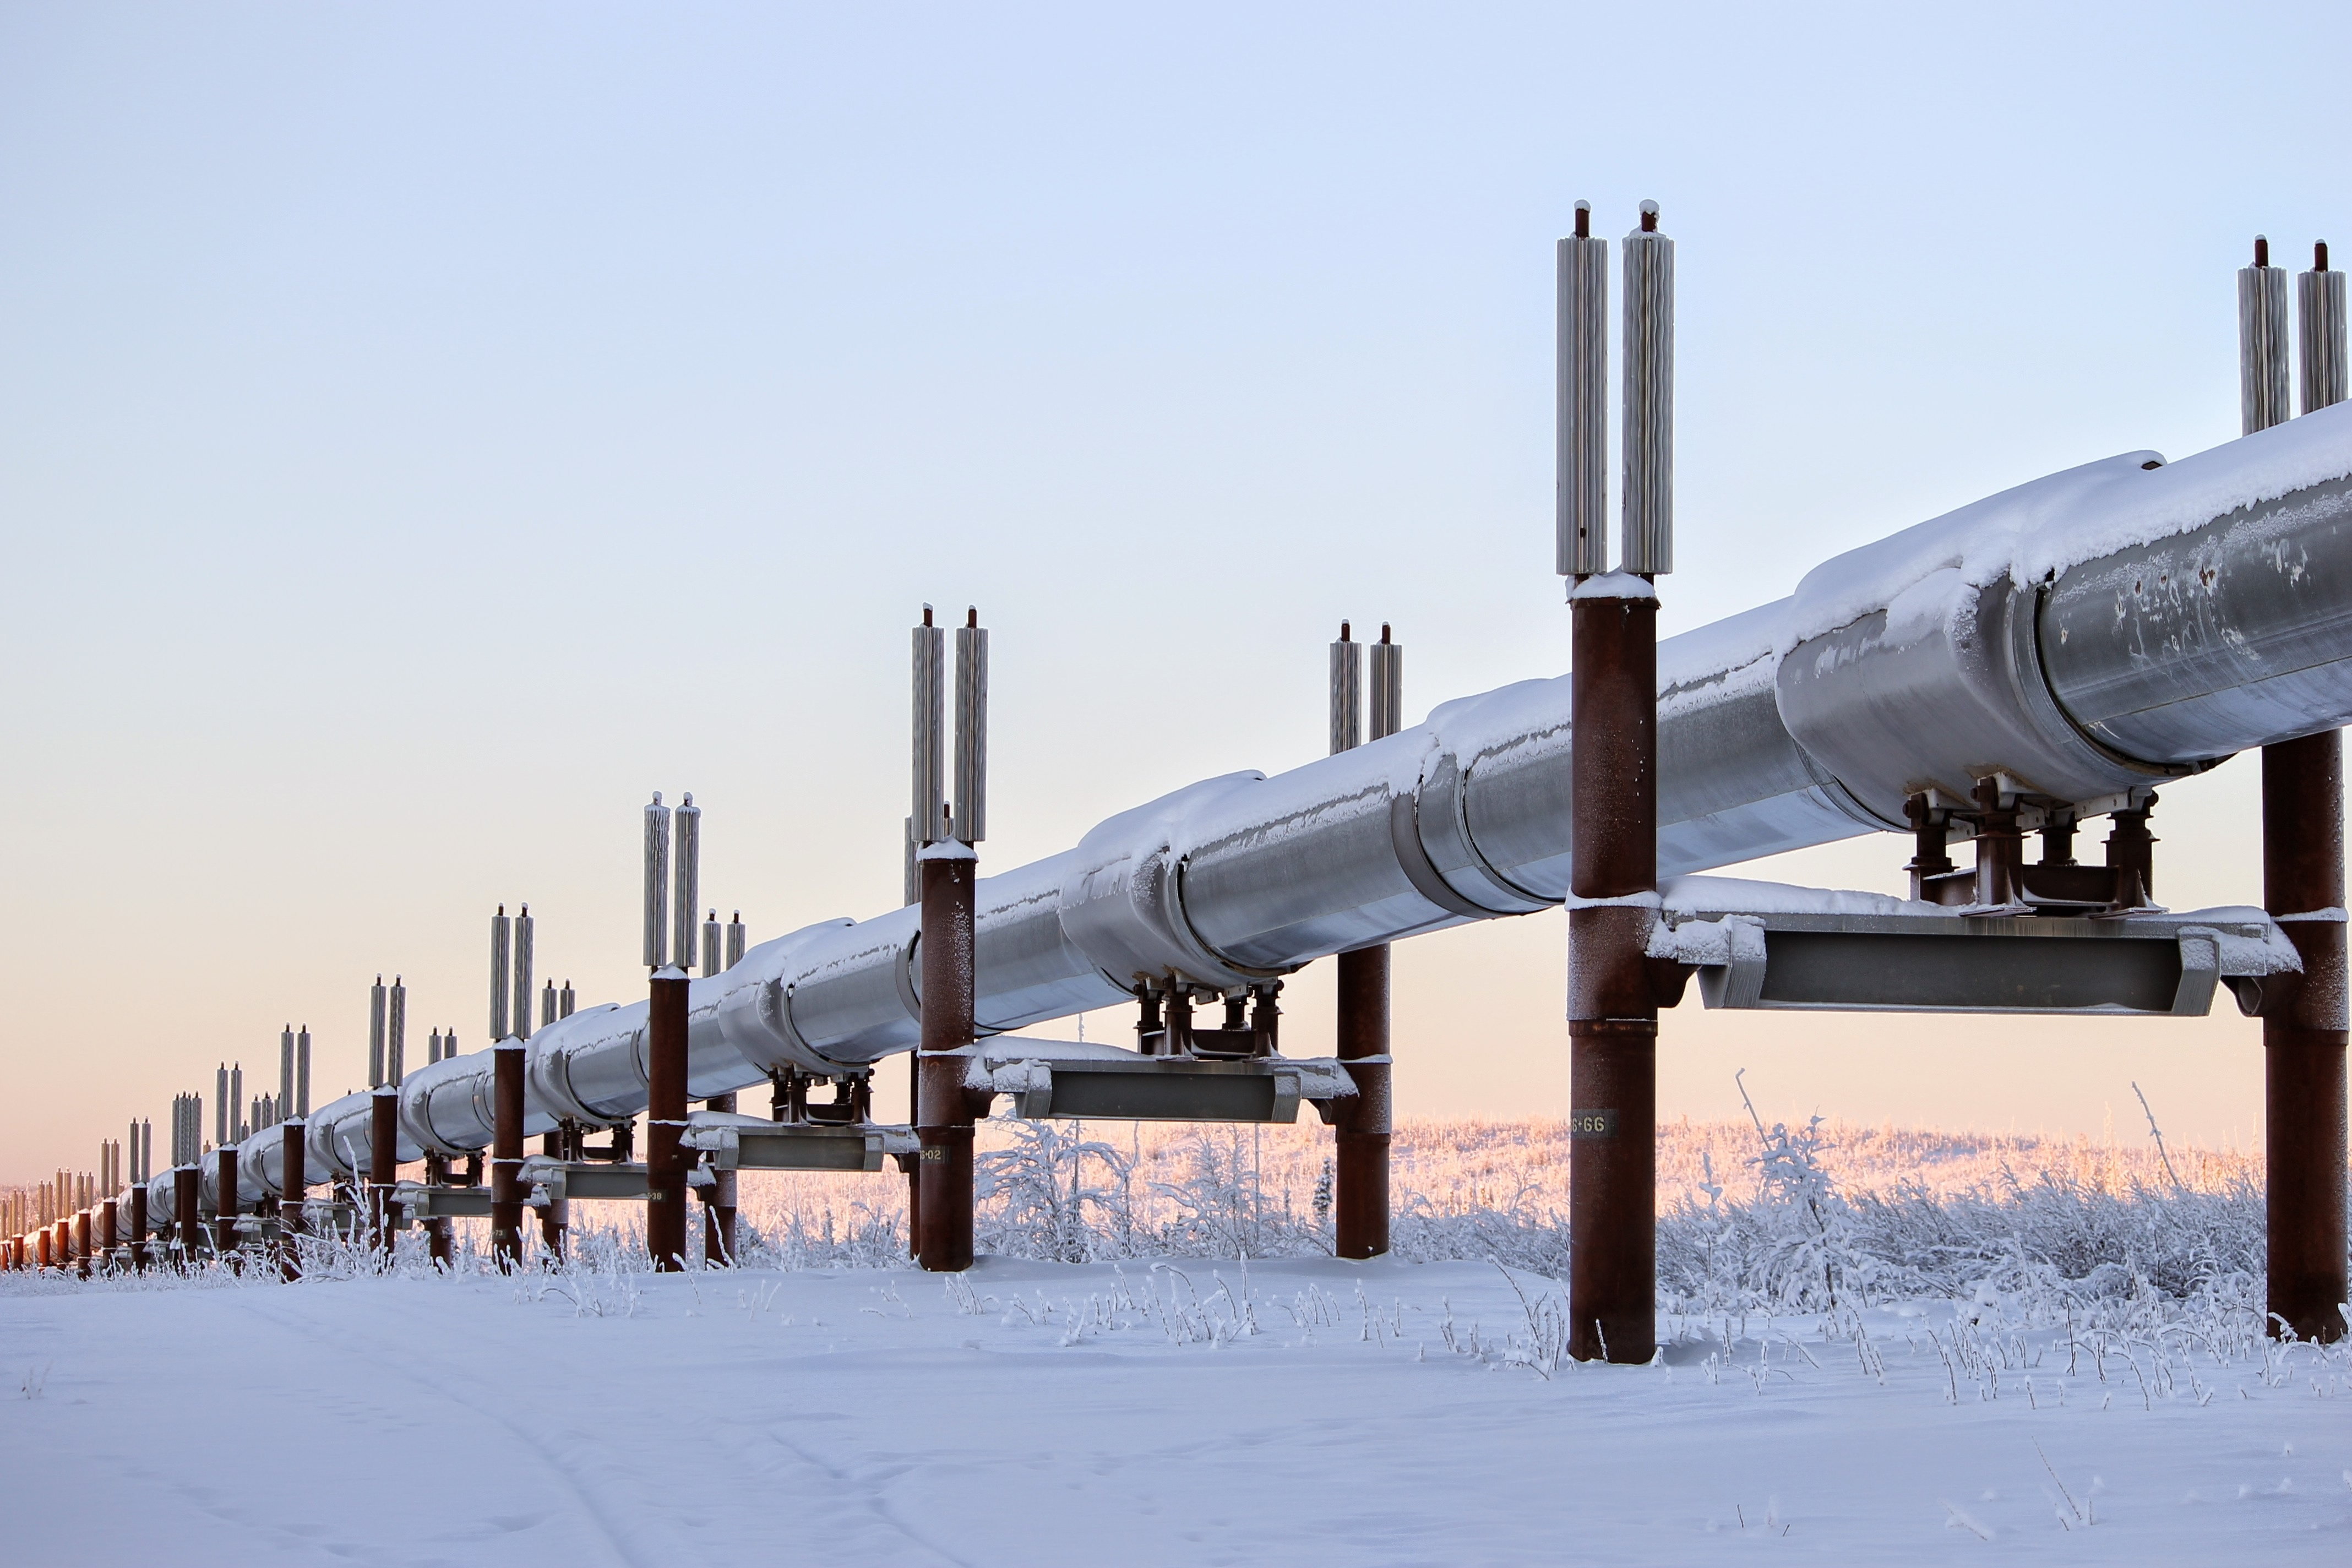
\includegraphics[width=0.55\textwidth]{Pipeline.jpg}


\end{minipage}\\[0.5em]
%
{\color{firstnamecolor}\rule{\textwidth}{.25ex}}
%
\begin{minipage}[t]{.4\textwidth}
	\raggedright%
	% {\bfseries {\color{firstnamecolor}
	\vspace*{1em}

	\small%
\end{minipage}
%
\hfill
%
\begin{minipage}[t]{.4\textwidth}
	\raggedleft % US style
	\today
	%April 6, 2006 % US informal style
	%05/04/2006 % UK formal style
\end{minipage}\\[2.2em]


{\bfseries \color{familynamecolor}{{\LARGE Energiepolitik im Baltikum -- Beispiel Erdgassektor}}}\\[0.75em]

\section*{\color{MidnightBlue}{\textsf{Besondere Eigenschaften von Gasmärkten}}}

\begin{itemize}
\item der Gassektor kann in die drei Segmente \textbf{Upstream} -- \textbf{Midstream} -- \textbf{Downstream} gegliedert werden

	\begin{itemize}
	\item \textbf{Upstream:} Exploration von Lagerstätten und Förderung von Erdgas\\
	\ding{225} sehr kostenintensive Tätigkeiten, die mit erheblichen unternehmerischen Risiken verbunden sind\\
	\ding{225} geographisch gebundene Geschäftsaktivität, die meist in einem Spannungsverhältnis mit Souveränitätsansprüchen von Nationalstaaten steht (meist sind Staatsunternehmen in diesem Bereich tätig: \textsl{Gazprom})\\
	\ding{225} private Förderunternehmen müssen beträchtliche 'Royalties' an Staaten zahlen

	\vspace{1cm}

	\item \textbf{Midstream:} Transport von Erdgas mittels Pipelines oder auf Schiffen in Form von Flüssiggas\\
	\ding{225} natürliche Monopole im Bereich der Infrastruktur

	\vspace{1cm}

	\item \textbf{Downstream:} Endverteilung, bzw. Vertrieb von Erdgas and Endverbraucher (Haushalte und Unternehmen)

	\vspace{1cm}

	\end{itemize}

\item beträchtliche \textbf{Sunk Costs} für Exploration Förderung und Transport von Erdgas\\
\ding{225} Föderanlagen und Pipelines können nach dem Bau nicht einfach versetzt werden\\
\ding{225} Sunk Costs können später nicht oder nur zu einem geringem Teil zurückgewonnen werden\\

\item \textbf{natürliche Monopole} im Midstream-Bereich:\\
\ding{225} hohe Sunk Costs, erhebliche Skalenerträge, hohe Markteintrittsbarrieren (\textsl{sehr hohe fixe Kosten im Verhältnis zu den variablen Kosten})\\
\ding{225} es macht wirtschaftlich nur Sinn, wenn ein Unternehmen die Infrastruktur für die Fernleitung von Erdgas bereitstellt und betreibt\\
\ding{225} diese Monopolsituation gibt dem Infrastrukturbetreiber erhebliche Marktmacht und somit politischen Einfluss


\item in Europa haben sich traditionell auf Gasmärkten sog. \textbf{vertikal integrierte Unternehmen} herausgebildet\\
\ding{225} da Energieversorgung meist als öffentliches Gut erachtet wurde, zumeist staatliche Monopolisten


\end{itemize}




\subsection*{\color{MidnightBlue}{\textsf{Gasmärkte in den baltischen Ländern}}}

\begin{itemize}

\item Estland, Lettland \& Litauen besitzen selbst keine nennenswerten Vorkommen an fossilen Brennträgern\\
\ding{225} sämtliche Primärenergie muss aus dem Ausland importiert werden\\
\ding{225} Baltikum ist eine \textbf{Energieinsel}

\item bis Anfang 2015 waren die baltischen Ländern gänzlich auf russisches Erdgas angewiesen, da keine Pipelines zu europäischen Gasnetzen bestehen

\item \textsl{Gazprom} hält an den staatlichen Energieversorgern \emph{Lietuvos dujos} und \emph{Lativjas G\={a}ze} große Anteile mit Kontrollmacht\\
\ding{225} Vize-Präsident von \emph{Lativjas G\={a}ze} Juris Savickis ist Ex-KGB Agent\\
\ding{225} politisch brisante Kombination aus Monopolsituation der Gasunternehmen und russischem Einfluss auf den baltischen Gasmärkten\\
\ding{225} der westliche Anteilseigner an \emph{Lietuvos dujos} und \emph{Lativjas G\={a}ze} ist die \textsl{E.ON Ruhrgas AG}, die traditionell gute Beziehungen zu ihren russischen Geschäftspartnern unterhält und Interesse an enger Kooperation mit Russland hat

\item russischer Einfluss ist potentiell vorhanden, jedoch nicht messbar (Interviews \& Aussage von Juris Savickis)

\item der Bau der Nordstream-Pipeline um das Baltikum herum gab den baltischen Ländern das Gefühl Spielball der großen Mächte Russland und Deutschland zu sein


\end{itemize}

\subsection*{\color{MidnightBlue}{\textsf{Gazprom}}}


\begin{itemize}

\item \textsl{Gazprom} ist mehrheitlich in der Hand der russischen Staates (Konzernchef Alexei Miller wird vom Kreml ernannt)

\item lange Geschichte von Lieferstopps an GUS-Staaten bei Erdgas (technische Gründe, wurden als Erklärung angeführt)\\
\ding{225} den Lieferunterbrechungen gingen häufig politische Entscheidungen voraus, die Russland nicht genehm waren


\item die Lieferstopps mit der Ukraine und Belarus hatten Zahlungsschwierigkeiten zur Ursache (\textsl{Technisches Gas})


\item Konzernstrategie \textsl{Gazproms}, das Midstream-Segment zu kontrollieren und im Ausland in das Downstream-Geschäft einzusteigen, macht wirtschaftlich Sinn\\
\ding{225} vertikale Integration downstream der Wertschöpfungskette ist ertragreicher als andersherum\\
\ding{225} die Gewinnung des Rohstoffes schafft im Verhältnis zum Kostenaufwand praktisch keinen Mehrwert der vermarktet werden könnte\\
\ding{225} Kalkül des Gaskonzern deckt sich häufig mit außenpolitischen Interessen Moskaus\\
\ding{225} Unterscheidung zwischen wirtschaftlicher und politischer Motivation ist nur schwer möglich

\end{itemize}



\subsection*{\color{MidnightBlue}{\textsf{Schwimmendes LNG-Terminal \textsl{Independence}}}}

\begin{itemize}

\item mit dem schwimmenden LNG-Terminal \textsl{Indepedence} verfügt Litauen über eine Alternative zu Erdgasimporten aus Russland

	\begin{itemize}
	
	\item litauisches Energieunternehmen \textsl{Klaip\.{e}dos Nafta} least das Schiff von der norwegischen Firma \textsl{Höegh LNG} für zunächst 10 Jahre
	
	\item jährlich können 4 Mrd. Kubikmeter Erdgas eingeführt werden, mehr der Jahresverbrauch von 2,7 Mrd.\\
	\ding{225} der Bedarf der baltischen Nachbarn kann auch zu 75 \% gedeckt werden\\
	\ding{225} hierzu müssen jedoch noch erforderliche Pipelines gebaut werden
	
	\item Liefervertrag mit der norwegischen \textsl{Statoil} auf 10 Jahre

	\end{itemize}

\ding{225} Verhandlungsmacht gegenüber Russland hat sich deutlich verbessert

\item Inbetriebnahme wurde von der litauischen Präsidentin \textsl{Dalia Grybauskait\.{e}} als Staatsakt gefeiert

\item Litauens Politik fühlt sich von Russland bei den Gaspreisen erpresst und hat bereits vor der EU-Kommission geklagt

\item LNG als Alternative zu russischen Importen ist ein finanzielle Frage, da Flüssiggas teurer als Erdgas

\item Litauen erschließt sich den weltweiten Gasmarkt und kann unter verschiedenen Anbietern wählen

\item langfristig wird der Weltmarktpreis für LNG sinken, da die Technik ausgereifter und günstiger wird, sowie mehr Kapazitäten entstehen

\item Litauen setzt dem Flüssiggasterminal weiterhin auf fossile Brennstoffe statt in erneuerbare Energien zu investieren



\end{itemize}

\newpage



\begin{figure}[htb]


  \begin{centering}
   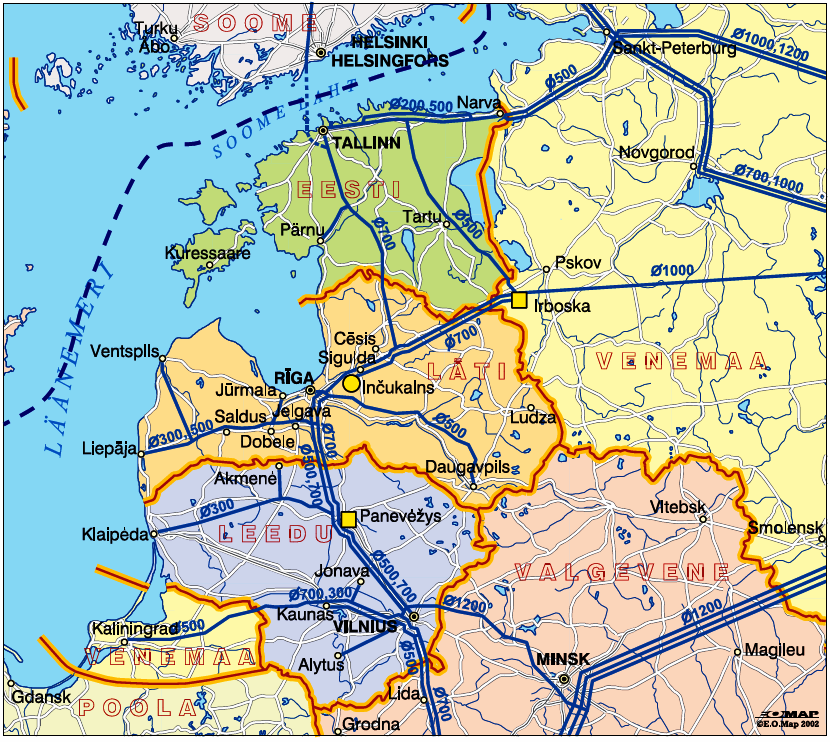
\includegraphics[width=1\textwidth]{Pipelines.png} % Herausgenommen: [scale=0.8]
    \caption{\textsf{Netz der Gaspipelines im Baltikum (\small{\textsl{Quelle:
	Eesti Gaas -\textcolor{MidnightBlue}{\url{http://www.eegas.com/estonia.htm}}})}}}

  \end{centering}

\end{figure}

\newpage

\section*{\color{MidnightBlue}{\textsf{Fragen an die Studenten}}}

\begin{enumerate}

\item Welche Bedeutung hat Energie für Gesellschaft und Staat? Welche Theorieschulen der IB bieten sich für die Erklärung von internationaler Energiepolitik an?

\item Wie würden Sie versuchen, politische und wirtschaftlicher Motivation voneinander zu unterscheiden?


\end{enumerate}



\end{document}